\section{Case Studies}\label{sec:eval}

In this section, we use both functional and imperative languages as host languages to illustrate the \appdiwchanged{flexibility and practicality} of Osazone. In the \appdiwchanged{first example}, we aim to show how a functional language is progressively extended with richer features by using primitive extension and monad extension, and specialized to DSLs using translation rules. In the second example, we aim to demonstrate the generality of our approach, presenting its applicability on imperative host languages.

% we will show the derived semantics which satisfies abstraction and how the evaluation of a DSL program is shown to the DSL users.
% The languages discussed in this section and their relation are shown in Fig. \ref{fig:langs},
%  where horizontal arrows represent meta-extensions and monad extensions,
%  and vertical arrows stand for specialization by translation rules.

\subsection{DSLs on Functional Host Languages}

The languages discussed in this section and their relationships are shown in Fig. \ref{fig:langs},
 where horizontal arrows represent primitive extensions and monad extensions,
 and vertical arrows stand for DSL definition by translation rules.

We have shown the syntax and semantics of \STLC, \textsc{Bool} (in Sec. \ref{sec:overview}), and \Func (in Sec. \ref{sec:host}).
We start with \STLC, a language with lambda calculus, integers, and Booleans.
From \STLC, we define \textsc{Bool} using translation rules.
With primitive extensions, we can extend \STLC{} to \STLCex{} by adding language constructs. % except references.
And then, we introduce a state monad \diwchanged{to support references}, getting \Func.
I/O can also be supported in \Func\ by adding a new language construct $\<print>$ via monad extension. For brevity, we skipped the discussion about this extension.

\begin{figure}
  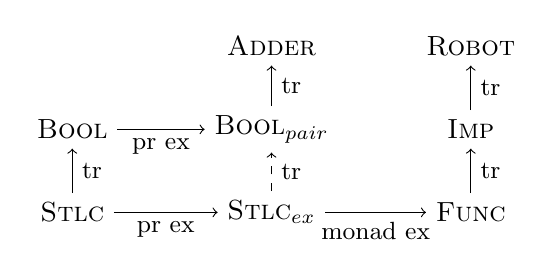
\begin{tikzpicture}[x=6pt,y=3pt,yscale=1,xscale=1]
%uncomment if require: \path (0,300); %set diagram left start at 0, and has height of 300

\node (STLC) at (-2,10) {\textsc{Stlc} };
\node (Bool) at (-2,20) {\textsc{Bool} };
\node (Boolp) at (10,20) {\textsc{Bool}$_\text{pair}$};
\node (Adder) at (10,30) {\textsc{Adder} };
\node (STLCex) at (10,10) {\textsc{Stlc}$_\text{ex}$};
\node (Ref) at (22,10) {\textsc{Func} };
\node (Imp) at (22,20) {\textsc{Imp} };
\node (Robot) at (22,30) {\textsc{Robot} };

\draw[->] (STLC) -> node[right] {\small tr} (Bool); 
\draw[->] (Bool) -> node[below] {\small pr ex} (Boolp);
\draw[->] (STLC) -> node[below] {\small pr ex} (STLCex);
% \draw[->] (STLC) -- node[below] {\small pr ex} (STLC-|STLCex) 
%  -> node[right] {\small tr} (STLCex);
\draw[->] (STLCex) -> node[below] {\small monad ex} (Ref); 
%\draw[->] (Ref) -> node[below] {\small monad ex (IO)} (RefIo);
\draw[->] (Ref) -> node[right] {\small tr} (Imp); 
\draw[->] (Imp) -> node[right] {\small tr} (Robot); 
\draw[->] (Boolp) -> node[right] {\small tr} (Adder); 
\draw[->, dashed] (STLCex) -> node[right] {\small tr} (Boolp); 
\end{tikzpicture}

  \caption{Languages Extended and Specialized from \STLC}
  \label{fig:langs}
\end{figure}

\subsubsection{Language \textsc{Adder}}

Consider that developers would like to
\diwchanged{
develop a DSL based on the \textsc{Bool} language, named \textsc{Adder},
which
}
supports $\<halfa>$ and $\<fulla>$ to simulate digital circuit. For example, in the language \textsc{Adder}, we have
\[ \<halfa>~\<true>~\<false> \Da (\<true>, \<false>). \]
However, they are not easily implemented by translation rules directly, because half-adder and full-adder will get the pair of sum and carry as the results. Pairs are demanded to build compound data structures now. Primitive extensions are used to make the host language support new data types.
In this example, developers add pair and projection to the language, and specify the evaluation (and typing) rules for each newly-defined language construct. Then developers get a new language $\textsc{Bool}_{\text{pair}}$ supporting pairs and projection. With the following translation rules, we can implement the DSL \textsc{Adder} that simulates half-adders and full-adders.
\begin{align*}
\<halfa>~e_1~e_2 & ->_d (e_1~\<xor>~e_2,e_1~\<and>~e_2) \\
\<fulla>~e_1~e_2~e_3 & ->_d (e_1~\<xor>~e_2~\<xor>~e_3, (e_1~\<xor>~e_2)~\<or>~(e_3~\<and>~(e_1~\<xor>~e_2)))
\end{align*}

The evaluation rules of $\<halfa>$, for example, are derived as follows:
\begin{gather*}
\inference{e_1\Da \<true> & e_2\Da \<true>}{\<halfa>~e_1~e_2 \Da (\<false>,\<true>)} \quad
\inference{e_1\Da \<true> & e_2\Da \<false>}{\<halfa>~e_1~e_2 \Da (\<true>,\<false>)} \\[1em]
\inference{e_1\Da \<false> & e_2\Da \<true>}{\<halfa>~e_1~e_2 \Da (\<true>,\<false>)} \quad
\inference{e_1\Da \<false> & e_2\Da \<false>}{\<halfa>~e_1~e_2 \Da (\<false>,\<false>)}
\end{gather*}
% At this time monad has not been introduced. 

%  implementing some languages based on \STLC. 
% Some of these language have been discussed.
% We start with \STLC, a language with lambda calculus and Boolean values.
% From \STLC, we define \textsc{Bool} using translation rules.
% By extending \textsc{Bool} with meta-extensions, we get $\textsc{Bool}_{\text{pair}}$ supporting pairs and projection.
% With two additional translation rules, we implement a DSL \textsc{Adder} that can simulate half adders and full adders.

\subsubsection{Language \textsc{Imp}}

Since we have added a store to \Func, we can now express programs that contain side effects. 
Taking \Func\ as the host language, we want to implement a reference-based imperative language \textsc{Imp}.
In \Func, the declarations and initial values of variables are necessary.
% For example, a legal \textsc{Imp} program and \Func\ program after translation are shown as follows:
For instance, a legal \Func\ program is shown as follows:
\[  \<let>~x=\<ref>~1~\<in>~x:=\ !x+1;\ !x \]
%In contrast, the following program is not permitted but is closer to general IMP programs:
Ideally, we want to write the corresponding DSL program in a more traditional IMP-like syntax:
\[ x:=1;x:=x+1. \]
We discuss why it is impossible to make the syntax of \textsc{Imp} exactly the same as traditional IMP-like language. Moreover, we define some other common language constructs for \textsc{Imp}.
% for convenience.

The declaration in the \textsc{Imp} language is a let-binding in \Func, where what is assigned must be a reference to some expression. In order to simulate the syntax of declaration in common imperative languages, we can define translation rule $\<var>$ as a syntactic sugar:
\[ \<var>~x=e_1; e_2 ->_d \<let>~x=\<ref>~e_1~\<in>~e_2 \]
This semicolon is used as part of the syntax of declaration, to ensure that $x$ is valid in $e_2$.

At first glance, this seems like a perfect translation. However, in an usual assignment statement, the left-hand side is a variable, denotes a location in the store (known as the L-value in the C-world) but any variable at the right-hand side refers to the value stored in it (known as the R-value in the C-world). We cannot distinguish these different occurrences by using translation rules.
% Regretfully, we are not able to simplify this by translation rules, 
As a result, explicit dereferences are required in \textsc{Imp} programs. % A solution is to distinguish such $x$ by the parser, and transform to $!x$ in abstract syntax tree automatically. To prevent confusion, we still write dereferences in the following discussion.

\begin{figure}
  \begin{align*}
    \<var>~x=e_1; e_2 & ->_d \<let>~x=\<ref>~e_1~\<in>~e_2 \\
    \<when>~e_1~e_2 & ->_d \<if>~e_1~e_2~() \\
    e_1 +\!\! = e_2 & ->_d e_1 := !e_1 + e_2 \\
    \<while>~e_1~\<do>~e_2~\<end> & ->_d ((\<fix>~(\lambda f.~\lambda x.~\lambda y.~\<if>~x~\<then>~(y; (f~x~y)_N)~\<else>~()))~e_1~e_2)_N
  \end{align*}
  \caption{Translation Rules for \textsc{Imp}}
  \label{fig:imp}
\end{figure}

Other language constructs in \textsc{Imp} are defined in Fig. \ref{fig:imp}. Note that we define $\<while>$ using the $\<fix>$ construct, because recursively defined translation rules are not allowed. {Note that} the translation rule does not satisfy assumption \ref{asm:tr_abs}, {because} $\<if>$ and sequencing are used in the non-abstract component of lambda abstraction. Using lambda lifting, we get the following two translation rules:
\begin{align*}
    \<body>~e~e_1~e_2 & ->_d \<if>~e_1~\<then>~e_2;(e~e_1~e_2)_N~\<else>~() \\
    \<while>~e_1~\<do>~e_2~\<end> & ->_d ((\<fix>~(\lambda f.~\lambda x.~\lambda y.~\<body>~f~x~y))~e_1~e_2)_N
\end{align*}
Those derived evaluation rules satisfy abstraction property with $\<body>,\<fix> \in \mathcal{S}$, shown in Fig. \ref{fig:while_rule}. 
Note that we do not applied rule of $\<body>$ recursively, since all the constructs in the expression are elements of $\mathcal{S}$.
As an instance of \textsc{Imp}, the following program is implemented to calculate the sum of 1 to 10.
\[ \<var>~n=1;\<var>~sum=0;\<while>~n < 11~\<do>~sum\ +\!\!=\ !n; n\ +\!\!=\ 1;\ !sum~\<end> \]

\begin{figure}
\begin{gather*}
  \inference{e_1 \Da_S \<true> & e_2 \Da_S () & e \Da_S \lambda x.~\lambda y.~e' & [x\mapsto e_1, y\mapsto e_2]e' \Da_S v}{\<body>~e~e_1~e_2 \Da_S v} \\[1em]
  \inference{e_1 \Da_S \<false> }{\<body>~e~e_1~e_2 \Da_S ()} \qquad
  \inference{\<body>~(\<fix>~(\lambda f.~\lambda x.~\lambda y.~\<body>~f~x~y))~e_1~e_2 \Da_S v}{\<while>~e_1~\<do>~e_2~\<end> \Da_S v}
\end{gather*}
    \caption{Derived Evaluation Rule of $\mathit{body}$ and $\mathit{while}$}
    \label{fig:while_rule}
\end{figure}

\subsubsection{Language \textsc{Robot}}

Based on \textsc{Imp}, we implement a DSL named \textsc{Robot}. The language assumes that a robot is located at some \diwchanged{initial coordinate} and users can control its movement or print out its position with commands. 
% In this example, we will emphasize the close property of translation rules. The goal of this language is to achieve simple control of robots in a two-dimensional plane.
A sample program of \text{Robot} is:
\[ \mathit{robot~5~5~\{ up, up, right, whereAmI, left, whereAmI \}} \]
where $\mathit{robot}~5~5~\{...\}$ declares a robot with an \diwchanged{initial coordinate} of $(5,5)$,
and the braces contain a series of commands to be executed on the robot, splitted by a comma.
Commands $\mathit{up},\mathit{right},\mathit{left}$ are used to control the movement of the robot
 and command $\mathit{whereAmI}$ will print current position.

As a natural idea, we \diwchanged{might} record the current position of the robot via the global variables $x$ and $y$. Then each command reads and manipulates global variables, and the comma is defined as sequencing. These language constructs are defined as follows:
\begin{align*}
  \<robot>~e_1~e_2~\{e\} & ->_d \<let>~x=\<ref>~e_1,y=\<ref>~e_2~\<in>~e \\
  e_1,e_2 & ->_d e_1;e_2 \\
  \<left> & ->_d x:=\ !x-1 \\
  \<whereAmI> & ->_d \<print>~!x; \<print>~!y
\end{align*}
where $x$ and $y$ are literal identifiers. \diwchanged{However,} under such definitions, the requirement of closed translation rules is not satisfied. \diwchanged{Because} variables without local bindings cannot be used directly in translation rules, it is necessary to pass the value of the variable as an argument to the language constructs or as an argument to a lambda abstraction. Hence, $\<left>$ should be expressed as
\[ \<left> ->_d λpos. ~(\<fst>~pos)~ \texttt{+=}~ (-1); pos, \]
where $pos$ has type $(\<Rf>~\<int>)\times (\<Rf>~\<int>)$.
Note that $\<left>$ returns $pos$ to keep passing on the ``global'' state.
Then, the comma operator is actually the composition of these functions.
Some other selected translation rules for \textsc{Robot} are given in Fig. \ref{fig:robot}.

\begin{figure}
  \begin{align*}
    \<robot>~e_1~e_2~\{e \} & ->_d e~(\<ref>~e_1,\<ref>~e_2) \\
    e_1,e_2 & ->_d λpos. ~e_2~(e_1~pos) \\
    \<left> & ->_d λpos. ~(\<fst>~pos)~ \texttt{+=}~ (-1); pos \\
    \<whereAmI> & ->_d λpos. ~\<print>~!(\<fst>~pos); \<print>~!(\<snd>~pos); pos
  \end{align*}
  \caption{Translation Rules for \textsc{Robot}}
  \label{fig:robot}
\end{figure}

Don't forget that because they are defined via lambda abstraction, lambda lifting is also necessary.

%%%%%%%%%%%%%%%%%%%%%%%%%%%%%%%%%%%%%%%%%%%%%%%%%%%%%%%%%%%%%%%%%%%%%%%%%%%%%%%%%%%%%%%

\subsection{DSLs on Imperative Host Languages}

Consider that we would like to implement a DSL to simulate finite-state machines, called \textsc{Fsm}.
We simplify the \diwchanged{setting} by using integers to represent states and symbols.
In this section, we will implement a language in which the programs look like this:
\begin{align*}
& \<automata>: \\
& \hspace{1em} \<input> ~ 5\ \{ r~0; r~1; r~0; r~1; r~0 \}; \\[-5pt]
& \hspace{1em} \<exec>\ \{ 0 \xrightarrow{0} 2; 0 \xrightarrow{1} 1; 
 1 \xrightarrow{0} 2; 1 \xrightarrow{1} 1; 
 2 \xrightarrow{0} 2; 2 \xrightarrow{1} 3; 
 3 \xrightarrow{0} 1; 3 \xrightarrow{1} 0; \}; \\
& \hspace{1em} \<enda>;\end{align*}
This machine has 4 states and 2 symbols in the alphabet.
The initial state is 0 (implicitly) and transition rules are defined after keyword $\<exec>$.
We use 5 symbols as input of this automaton declared by $\<input>$, 
and the \diwchanged{evaluation of the} program should tell us the final state.

To implement this, we choose a simplified version of \Cminor{} \cite{cminor} as the host language.
In our problem, we only need to define the main function, so we can ignore \diwchanged{language features} such as the function call stack.
In addition, types and memory models are not our focus. 
Therefore, we assume that only integers are stored in the heap, meaning that the offset of a pointer is fixed.
% In this language, we need to maintain the global memory state and the environment mapping local variables to values.
% Similarly, we use state monad to follow them.
% In addition, incorrect store or load will cause diverging computation, which can be described by maybe monad.
% Through monad transformer, we can combine the above two monads as one monad, denoted by $m$.

The DSL program will be translated into the execution of the main function.
In \Cminor{}, a function is defined by a list of parameters (null for main function), 
 a list of local variables, and a body statement.
Defining variables in the body is not allowed.
Therefore, to provide the translation rules for the DSL,
we need to identify the local variables that will be used in \textsc{Fsm}.
% The language construct $\<automata>$ in \textsc{Fsm}, which will be translated into a \Cminor{} program,
% must declare these local variables.
The translation rule of $\<automata>$ is defined as follows:
\[ \<automata>:~stmt ->_d \texttt{main() \{ var n,syms,i,st; $stmt$ \}} \]
where $stmt$ is the body of main function; 
$n$ is the number of input symbols; 
$syms$ is the pointer pointing to the first cell of input symbols;
$st$ is current state;
and $i$ is auxiliary variable for iteration.

The language constructs $\<input>$ and $r$ are used to record the input symbols.
The $\<input>$ \diwchanged{construct} first initializes local variable $n$ and $i$, and then allocates the requested size.
After that, $r$ is used to store the inputs.
The translation rules of $\<input>$ and $r$ are defined as:
\begin{align*}
  \<input>~expr~stmt & ->_d \texttt{n := }expr\texttt{; i := 0; syms := malloc(n); } stmt \\
  r~expr & ->_d \texttt{[syms + i] := } expr \texttt{; i := i + 1;}
\end{align*}
In RHS, statements include assignment to local variable (with shape \texttt{ident := expr}, memory stores (with shape \texttt{[$expr$] := $expr$}) and sequencing.
Expressions include reading local variables, constants, \diwchanged{binary} operations, and function calls.
In \Cminor{}\ , \texttt{malloc} is seen as an external function, while we use it as a primitive operation, 
which takes the size as argument and returns the address of a
\diwchanged{newly allocated memory block with the requested size}.

The \textsc{FSM} processes input through language construct $\<exec>$. 
It repeatedly changes the state based on the current input until all input characters are consumed.
The body of $\<exec>$ consists of a list of transfer rules and each of them will be translated into an \texttt{if} statement.
If one of the rule is matched, there should be a \texttt{continue}.
And if there is no rule that can be matched, the state will be set as $-1$ and the loop should exit through \texttt{break}. 
In \Cminor{}, only infinite looping is introduced.
And \texttt{break} and \texttt{continue} are implemented with blocks and \texttt{exit} statements.
We use $\texttt{exit}~n$ to leave $(n+1)$ enclosing blocks.
For example, in \Cminor{}, $\texttt{while}~e~s$ is written as 
\[ \texttt{block \{ loop \{ if !$e$ then exit 0; block \{ $s$ \} \}\}}. \]
Note that the braces here are used to enclose a group of statements connected by sequence, 
while a block is used with the \texttt{block} language construct.
In $s$, if there are no nested blocks, \texttt{continue} can be written as \texttt{exit 0} and \texttt{break} \diwchanged{can be written as} \texttt{exit 1}.
Based on the above discussion, we can define the following translation rules:
\begin{align*}
    \<exec>~stmt & ->_d \texttt{i := 0; block \{ loop \{ if (i == n) exit 0; } \\ 
    & \qquad\qquad \texttt{block \{}~stmt~\texttt{; st := -1; exit 1; \}\}\} }  \\
    expr_1 \xrightarrow{expr} expr_2 & ->_d \texttt{if (st == } expr_1 \texttt{ \&\& load (syms + i) == } expr \texttt{) \{} \\
    & \qquad\qquad \texttt{st := } expr_2 \texttt{; i := i + 1; exit 0; \}}
\end{align*}

Finally, $\<enda>$ is used to print the final state.
\[ \<enda> ->_d \texttt{print(st); return 0;} \]
where \texttt{print} is an external function in \Cminor{} and \texttt{return} statement will finish the function execution.

Next, we will discuss the semantics of \Cminor{}.
We use a monad to describe the changes in the global heap and local environment.
Due to diverging computations caused by incorrect storage and retrieval, 
and the \diwchanged{potential} use of undefined variables, 
we also need to introduce the maybe monad.
We combine the above two monads with the I/O monad using a monad transformer and denote \diwchanged{the combined monad} as $m$.

The evaluation of an expression $expr \Da_m val$ does not cause changes in the environment or memory, 
but it may read the value of variables or pointed-to values of pointers from the state.
Statements evaluate to \textit{outcomes} $stmt \Da_m out$, indicating how afterwards execute. 
There are three types of outcomes: \texttt{norm} (for normal, continuing in sequence), $\texttt{ex}~n$ (for exit, terminating the $n+1$ enclosing blocks), $\texttt{ret}~val$ (for return).
Some evaluation rules of expressions and statements are shown in Fig. \ref{fig:cminor}.
One thing to note here is the \texttt{loop} construct.
By using $later$, We transform the recursion in the evaluation rule of the \texttt{loop} construct into a meta-function call to satisfy assumption \ref{asm:host_abs}.
Clearly, the meta-function $later(stmt)$ returns the evaluation result of $stmt$.
Furthermore, \diwchanged{because} $stmt$ is used as an argument in the meta-function, 
it is a non-abstract component of \texttt{loop $stmt$}.
All these evaluation rules and meta-functions obey the assumptions.

\begin{figure}

\addtolength{\jot}{5pt}
\begin{gather*}
\noalign{\raggedright \hspace{2em} Expression: $expr \Da_m val$}
\inference{\mathit{get}(x) =>_m val}{x \Da_m val} \quad
\inference{expr\Da_m addr & \mathit{load}(addr)=>_m val }{\texttt{load}~expr \Da_m val } \\
\noalign{\raggedright \hspace{2em} Statement: $stmt \Da_m out$}
\inference{ expr\Da_m val & update(x, val)}{x := expr \Da_m \texttt{norm} } \\
\inference{ expr_1\Da_m addr & expr_2 \Da_m val & store(addr, val)}{ [expr_1] := expr_2 \Da_m \texttt{norm} } \\
\inference{ stmt_1\Da_m \texttt{norm} & stmt_2\Da_m out }{stmt_1;stmt_2 \Da_m out } \quad
\inference{ stmt_1\Da_m out & out \ne \texttt{norm} }{stmt_1;stmt_2 \Da_m out } \\
\inference{ stmt \Da_m \texttt{norm} & later(\texttt{loop}~stmt) =>_m out }{ \texttt{loop}~stmt \Da_m out } \quad
\inference{ stmt \Da_m out & out \ne \texttt{norm} }{ \texttt{loop}~stmt \Da_m out } \\
\inference{ stmt \Da_m \texttt{ex}~0 }{ \texttt{block}~stmt \Da_m \texttt{norm} } \quad
\inference{ stmt \Da_m \texttt{ex}~n }{ \texttt{block}~stmt \Da_m \texttt{ex}~(n-1) } \\
\inference{ stmt \Da_m out & out \ne \texttt{ex}~n }{ \texttt{block}~stmt \Da_m out } \quad
\inference{}{ \texttt{exit}~n \Da_m \texttt{ex}~n } \quad
\inference{ expr \Da_m val }{ \texttt{return}~expr \Da_m \texttt{ret}~val } \\
\noalign{\raggedright \hspace{2em} Main Function: $\mathit{func} \Da_m val$}
\inference{ \mathit{newEnv}(vars) & stmt \Da_m \texttt{ret}~val }{\texttt{main() \{ var $vars$; $stmt$ \} } \Da_m val }
\end{gather*} 

\caption{Selected Evaluation Rules of \Cminor{}}
\label{fig:cminor}
\end{figure}

For the translation rules, we need to show that they satisfy our closed translation requirement.
In \Cminor{}, all variable assignments and reads are done through meta-functions, 
which means that undefined variables will fail at run-time of the meta-function.
In the derived evaluation rules, variables can be read dynamically.
Hence, in the translation rules, it is not necessary to perform local binding for variables to achieve correct semantics lifting.
But correspondingly, hygiene cannot be guaranteed as a result.
To satisfy assumption \ref{asm:tr_abs}, \texttt{exec} needs to be split into two translation rules:
\begin{align*}
\texttt{step}~stmt & ->_d \texttt{if (i == n) exit 0; block \{}~stmt~\texttt{; st := -1; exit 1; \} }  \\
\<exec>~stmt & ->_d \texttt{i := 0; block \{ loop \{ \texttt{step}~stmt \}\} }  \\
\end{align*}
Their semantics can be statically derived and will not be elaborated here.

% \begin{figure}
%     \centering
%     \begin{verbatim}
%     int main() { 
%       var n, syms, i, st; 
%       n := 5; i := 0; syms = malloc(5);  // input 5
%       [syms + i] := 0; i := i + 1;  // r 0
%       [syms + i] := 1; i := i + 1;  // r 1
%       ...
%       i := 0; block { loop {  // exec
%         if (i == n) exit 0; block {
%           if (st == 0 && load (syms + i) == 0) {
%             st := 2;
%             i := i + 1;
%             exit 0;
%           }
%           ...
%           st := -1; exit 1;
%         }
%       } }
%       print(st); return 0;
%     }
%     \end{verbatim}
%     \caption{Caption}
%     \label{fig:my_label}
% \end{figure}


% From another dimension, we start with meta-extensions on \STLC.
% Language constructs pairs, sums, fixpoints and lists,
%  introduced in Chapter 11 of Types and Programming Languages\cite{tapl} are tested.
% And let bindings and ascription are implemented by translation rules.
% We name the new language as \STLCex.
% In this language, we will talk about the impact of fixpoints on abstraction.

% Then, we introduce reference and I/O by monad extension, getting \textsc{Ref}.
% Taking \textsc{Ref} as the host language,
%  we implement an imperative language \textsc{Imp}.

% The point we should care about in \textsc{Imp} is that,
%  recursive translation rules are declared in $\<while>$.
% As an extension of our framework,
%  we will discuss weak-abstraction semantics derivation.
%
% After that, we make \textsc{Ref} support I/O, getting \RefIO.
% Based on \textsc{Imp}, we implement a DSL named \textsc{Robot}.
% The language assumes that a robot is located at some starting coordinates,
%  and users can control its movement, or print out its position with commands.
% In this example, We will talk about how to access ``global variables'' in the translation rules.

% \subsection{\STLCex: Fixpoint}\label{sec:fix}

% Fixpoint is a common approach to implement recursion in functional programming language.
% As a primitive language construct, the evaluation rule and typing rule of $\<fix>$ are specified:
% \begin{align*}
%   \ctr{Fix}{ \<fix>~e} & \cqq \Let{λx\!:\!t.e_1}{\EE{e}} \EE{e_1[\<fix>~(λx\!:\!t.e_1)/x]}
%   % \TT{\<fix>~e} & \cqq \TT{e}:(t_1->t_2\mid t_1=t_2 |> t_1). 
% \end{align*}

% Since an expression with substituion are evaluated,
%  the evaluation rule is not structural.
% And as mentioned above, nonstructural evaluation rule should be considered how to maintain abstraction.
% % In fact, thanks to lambda lifting and the existing discussion on substitution, fixpoint is easy to solve.
% % However, unfolding according to the rules of $\<fix>$ leads to non-termination of the algorithm.
% We assume that fix can be preserved in the DSL--for a language that contains recursion is straightforward.
% We add the following rule to the $\dd$:
% \[ \dd(\HH{\<fix>~\mexp}) = \Let{λx\!:\!t.e_1}{\dd(\HH{\mexp})} \HH{\<fix>~(λx\!:\!t.e_1)} \]
% where we do not expand the substitution with fixpoint resursively.
% The above rule is equivalent to the extended rule in Section \ref{sec:alg-ex}, but the $\<fix>$ is kept in the rule for readability.

% \begin{example}
% \[ \<iseven> => \<fix>~(λie\!:\!int->bool.~λx\!:\!int.~\<if>~(x=lit~0)~\<true>~(\<if>~(x=lit~1)~\<false>~(ie~(x-lit~2)))) \]
  
% The first step is lambda lifting. The following translation rules are generated.
% \begin{align*}
%   \<iseven>'~e_1~e_2 & => \<if>~(e_2=lit~0)~\<true>~(\<if>~(e_2=lit~1)~\<false>~(e_1~(e_2-lit~2))) \\
%   \<iseven> & => \<fix>~(λie\!:\!int->bool.~λx\!:\!int.~\<iseven>'~ie~x)
% \end{align*}

% The evaluation rules of language constructs used by $\<iseven>'$ all have structural semantics.
% So the evaluation rule of $\<iseven>'$ is also structural.
% The evaluation rule of $\<iseven>$ can be derived by:
% \begin{align*}
%   & \ctr{IsEven}{\<iseven>} \\
%   \cqq~ & \dhl{\HH{\<fix>~(λie\!:\!int->bool.~λx\!:\!int.~\<iseven>'~ie~x)}} \\
%   =~ & \Let{λx'\!:\!t.e}{\dhl{\HH{λie\!:\!int->bool.~λx\!:\!int.~\<iseven>'~ie~x}}} \HH{\<fix>~(λx':t.e)} \\
%   =~ & \HH{\<fix>~(λie\!:\!int->bool.~λx\!:\!int.~\<iseven>'~ie~x)}
% \end{align*}
% Because of lambda lifting, $\<iseven>'$ is a DSL construct. The abstraction property holds.
% \end{example}



% \subsection{\textsc{Imp}: Recursive Translation Rules}\label{sec:while}

% Our \textsc{Imp} language is defined by translation rules based on \textsc{Ref},
%  which means the use of variables should be reference-based.
% Therefore, the syntax of \textsc{Imp} here is slightly different from the general language.
% First, the declarations and initial values of variables are necessary.
% For example, a legal \textsc{Imp} program is
% \[ \<let>~x=\<ref>~1~\<in>~x:=!x+1; !x \]
% And $x:=1;x:=x+1;x$ is not permitted for $x$ not in scope.
% Also, we find that what is assigned in the declaration must be a reference to some expression.
% In order to simulate the syntax of declaration in common imperative language,
%  we can define syntactic sugar $\<var>$ shown in Fig. \ref{fig:imp}.
% The semicolon is used as part of the syntax of the declaration, to ensure that $x$ is valid in $e_2$.

% Second, in \textsc{Imp}, the left-hand side of an assignment must be a variable
%  and the any variable at right-hand side refers to the value stored in it (a location).
% Regretfully, we are not able to simplify this by translation rules,
%  and explicit dereferences are essential.
% A solution is to distinguish such $x$ by the parser, and transform to $!x$ in abstract syntax tree automatically.
% We still write dereferences in the following discussion.

% \begin{figure}
%   \begin{align*}
%     \<var>~x=e_1; e_2 & => \<let>~x=\<ref>~e_1~\<in>~e_2 \\
%     \<when>~e_1~e_2 & => \<if>~e_1~e_2~() \\
%     e_1 +\!\! = e_2 & => e_1 := !e_1 + e_2 \\
%     \<while>~e_1~\<do>~e_2~\<end> & => \<if>~e_1~(e_2; \<while>~e_1~\<do>~e_2~\<end>)~()
%   \end{align*}
%   \caption{Translation Rules for \textsc{Imp}}
%   \label{fig:imp}
% \end{figure}

% Some other common language constructs in \textsc{Imp} are defined in Fig. \ref{fig:imp}.
% But $\<while>$, whose definition does not satisfy requirement \ref{req:no-recursion}, is our concern.
% By the algorithm extension of Section \ref{sec:alg-ex}, we have
% \begin{align*}
%   & \ctr{While}{\<while>~e_1~\<do>~e_2~\<end>} \\ 
%   \cqq~~ & \dhl{\EE{\<if>~e_1~(e_2; \<while>~e_1~\<do>~e_2~\<end>)~()}} \\
%   =~~ & \EE{e_1}:\branch{
%         \<true> |> \Let{()}{\EE{e_2}} \dhl{\EE{\<while>~e_1~\<do>~e_2~\<end>}} \\&
%         \<false> |> ()
%     } \\
%   =~~ & \EE{e_1}:\branch{
%       \<true> |> \Let{()}{\EE{e_2}} \EE{\<while>~e_1~\<do>~e_2~\<end>} \\&
%       \<false> |> ()
%   }
% \end{align*}
% Consider that we discard this step of expansion, the evaluation rule of $\<while>$ can be derived as follows, 
%  which is not structural but correct:
% \[ 
%   \ctr{While}{\<while>~e_1~\<do>~e_2~\<end>} \cqq \EE{e_1}:\branch{
%     \<true> |> \Let{()}{\EE{e_2}} \EE{\<while>~e_1~\<do>~e_2~\<end>} \\&
%     \<false> |> ()
%   } 
% \]
% Because $\<while>$ itself is a language construct in the DSL,
%  we can think of it as satisfying abstraction if we keep it in the evaluation rule.

% The more serious problem is the type derivation.
% It is reasonable that $\<while>$ has a recursive evaluation,
%  but the typing of $\<while>$ should not be.
% If the above approach is applied, an error typing rule is generated:
% \begin{align*}
%   \TT{\<while>~e_1~\<do>~e_2~\<end>} \cqq~
%   & \Let{\<bool>}{\TT{e_1}} \Let{\<unit>}{\TT{e_2}} \\
%   & \Let{t_2}{\TT{\<while>~e_1~\<do>~e_2~\<end>}} \<unit>:(t_3 \mid t_2=t_3 |> t_2)
% \end{align*}
% In this instance, the typing rule must be specified manually.

% More problem arise when \textsc{Imp} is used as a host language.
% When a language construct is translated to $\<while>$,
%  abstraction is difficult to guarantee.
% For example, $\<for>$ can be defined as follows, but we cannot derive an evaluation rule without $\<while>$.
% \[ \<for>~(e_1;e_2;e_3)~\<do>~e_4 => e_1;\<while>~e_2~\<do>~(e_4;e_3)~\<end> \]



% \subsection{\textsc{Robot}: Access to Global Variables}

% The goal of this language is to achieve simple control of robots in a two-dimensional plane.
% A sample program of \text{Robot} is:
% \[ \mathit{robot~5~5~\{ up, up, right, whereAmI, left, whereAmI \}} \]
% where $\mathit{robot}~5~5\{...\}$ declares a robot with a starting point of $(5,5)$,
% and the braces contain a series of commands to be executed on the robot, splitted by comma.
% Some commands are used to control the movement of the robot,
%  and command $\mathit{whereAmI}$ will print current position.

% As a natural idea, we record the current position of the robot via the global variables $x$ and $y$.
% Then each command reads and manipulates global variables,
%  and comma is defined as sequencing.
% These language constructs are defined as follows:
% \begin{align*}
%   \<robot>~e_1~e_2~\{e\} & => \<let>~x=\<ref>~e_1,y=\<ref>~e_2~\<in>~e \\
%   e_1,e_2 & => e_1;e_2 \\
%   \<left> & => x:=\ !x-1 \\
%   \<whereAmI> & => \<print>~!x; \<print>~!y
% \end{align*}
% where $x$ and $y$ are literal identifiers.
% But requirement \ref{req:close} is not satisfied.
% Since variables without local bindings cannot be used directly in translation rules,
%  it is necessary to pass the value of the variable as an argument to the language constructs or as an argument to a lambda abstraction.
% Hence, $\<left>$ can be expressed as
% \[ \<left> => λpos:(\<Rf>~\<int>)\times (\<Rf>~\<int>). ~(\<fst>~pos)~ \texttt{-=}~ 1; pos \]
% Note that $\<left>$ returns $pos$ to keep passing on the ``global'' state.
% Then, the comma operator is actually the composition of the functions.
% Some selected translation rules for \textsc{Robot} are given in Fig. \ref{fig:robot}.

% \begin{figure}
%   \begin{align*}
%     \<robot>~e_1~e_2~\{e\} & => e~(\<ref>~e_1,\<ref>~e_2) \\
%     e_1,e_2 & => λpos:(\<Rf>~\<int>)\times (\<Rf>~\<int>). ~e_2~(e_1~pos) \\
%     \<left> & => λpos:(\<Rf>~\<int>)\times (\<Rf>~\<int>). ~(\<fst>~pos)~ \texttt{-=}~ 1; pos \\
%     % \<right> & => λpos:(\<Rf>~\<int>)\times (\<Rf>~\<int>). ~(\<fst>~pos)~ \texttt{+=}~ 1; pos \\
%     % \<down> & => λpos:(\<Rf>~\<int>)\times (\<Rf>~\<int>). ~(\<snd>~pos)~ \texttt{-=}~ 1; pos \\
%     % \<up> & => λpos:(\<Rf>~\<int>)\times (\<Rf>~\<int>). ~(\<snd>~pos)~ \texttt{+=}~ 1; pos \\
%     \<whereAmI> & => λpos:(\<Rf>~\<int>)\times (\<Rf>~\<int>). \<print>~!(\<snd>~pos); \<print>~!(\<fst>~pos); pos
%   \end{align*}
%   \caption{Translation Rules for \textsc{Robot}}
%   \label{fig:robot}
% \end{figure}

